
\documentclass[%
onecolumn, notitlepage,
%superscriptaddress,
%groupedaddress,
%unsortedaddress,
%runinaddress,
%frontmatterverbose, 
%preprint,
%showpacs,preprintnumbers,
%nofootinbib,
%nobibnotes,
%bibnotes,
 amsmath,amssymb,
 aps,
%pra,
%prb,
%rmp,
%prstab,
%prstper,
%floatfix,
]{article}
\usepackage[
top    =2.5cm,
bottom = 2.5cm,
left   = 1.5cm,
right  = 1.5cm]{geometry}
%\usepackage{amsmath}
%\usepackage[tbtags]{amsmath}
\usepackage{graphicx}% Include figure files
\usepackage{dcolumn}% Align table columns on decimal point
\usepackage{bm}% bold math
\usepackage{mathtools}
\usepackage{physics}
\usepackage{natbib}
\usepackage{varwidth}
\usepackage{amsmath}
\usepackage{amssymb}		
\usepackage{fancyhdr}
\usepackage{float}
\usepackage[usenames, dvipsnames]{color}
\usepackage{tikz} 
\usepackage{ltxgrid}
\usetikzlibrary{shapes,arrows,positioning,automata,backgrounds,calc,er,patterns}
\usepackage{tikz-feynman}
\tikzfeynmanset{compat=1.0.0}
\usetikzlibrary{decorations.shapes}
\tikzset{decorate sep/.style 2 args=
{decorate,decoration={shape backgrounds,shape=circle,shape size=#1,shape sep=#2}}}
%\usepackage{tikz,newtxmath}
\usetikzlibrary{arrows,decorations.markings}
\usepackage[pdfencoding=auto]{hyperref}
\usepackage[utf8x]{inputenc} 
\usepackage{accents}

\usepackage{moreverb}		
\usepackage{listings}	

\usepackage[T1]{fontenc}
\usepackage{lmodern}
\usepackage{textcomp}
%\usepackage{pdflscape}
\usepackage{rotating}
\usepackage{color}
\usepackage{enumitem, xcolor}
\definecolor{MancPurple}{RGB}{93,42,122}
\definecolor{MancYellow}{RGB}{252,207,32}
\definecolor{Orange2}{RGB}{255,102,0}
\newcommand*{\dt}[1]{%
  \accentset{\mbox{\large\bfseries .}}{#1}}

\definecolor{testcolour}{rgb}{0.149019,0,0.439215}
\hypersetup{colorlinks=true,citecolor=testcolour ,urlcolor=testcolour,linkcolor=testcolour,filecolor=testcolour}
\pagestyle{fancy}
\fancyhf{}
%\fancyhead[LE,RO]{Share\LaTeX}
\fancyhead[RE,LO]{\textsc{MPhys $|$ PWFA}}
\fancyfoot[CE,CO]{\leftmark}
\fancyfoot[LE,RO]{\thepage}
 \newcommand*{\Scale}[2][4]{\scalebox{#1}{$#2$}}
\renewcommand{\headrulewidth}{2pt}
\renewcommand{\footrulewidth}{1pt}
\DeclareMathOperator{\sinc}{sinc}
\newcommand{\fvec}[1]{\underaccent{\Scale[1]{\sim}}{#1}}
\fancypagestyle{firstpage}{%
  \fancyhf{}
\fancyhead[LE,RO]{ \textsc{OSCAR JAKOBSSON $|$ 2018}}
\fancyhead[RE,LO]{\textsc{MPhys $|$ PWFA}}
\fancyhead[CE,CO]{\textsc{RESEARCH DIARY}}
\fancyfoot[LE,RO]{\thepage}
}
\usepackage{accents}
 \DeclareMathAccent{\wtilde}{\mathord}{largesymbols}{"65}
\usepackage{hyperref}

\newenvironment{tightcenter}{%
  \setlength\topsep{0pt}
  \setlength\parskip{0pt}
  \begin{center}
}{%
  \end{center}
}

\def\Xint#1{\mathchoice
   {\XXint\displaystyle\textstyle{#1}}%
   {\XXint\textstyle\scriptstyle{#1}}%
   {\XXint\scriptstyle\scriptscriptstyle{#1}}%
   {\XXint\scriptscriptstyle\scriptscriptstyle{#1}}%
   \!\int}
\def\XXint#1#2#3{{\setbox0=\hbox{$#1{#2#3}{\int}$}
     \vcenter{\hbox{$#2#3$}}\kern-.5\wd0}}
\def\ddashint{\Xint=}
\def\dashint{\Xint-}

\let\oldhat\hat
\renewcommand{\hat}[1]{\oldhat{{#1}}}
\renewcommand{\vec}[1]{\mathbf{#1}}


\def\dbar{{\mathchar'26\mkern-12mu \mathrm{d}}} 

\begin{document}

%\preprint{APS/123-QED}
\thispagestyle{firstpage}
\begin{minipage}{0.7\textwidth}
\vspace{-5pt}
\noindent \textbf{Project:} A compact plasma beam dump for next generation particle accelerators.\\
\noindent \textbf{Supervisor:} Dr. Guoxing Xia.\\ 
\noindent \textbf{Duration:} 24 Weeks, 2018-19.\vspace{-19pt}\\
\begin{tabbing}
\textbf{Location:}  \=The University of Manchester,\\
\>Cockcroft Accelerator Group,\\
\>Manchester, UK.
\end{tabbing}
\end{minipage}


\begin{figure}[h]
\vspace{-95pt}\hspace{0.85\textwidth}
\includegraphics[scale=0.4]{ManchesterCrest.pdf} 
\end{figure}\vspace{-35pt}
\noindent\rule{0.72\textwidth}{0.4pt}\\
\\
\noindent \textbf{Week 1}
\begin{itemize}
\item[\textcolor{MancPurple}{\textbullet}]  First meeting with Guoxing: Discussed project outline, necessary background reading and the \texttt{EPOCH} software. Received documents from Guoxing: LFWA PhD thesis \citep{Chou2016}, PWFA and beam dump papers \citep{Bonatto2015,Bonatto2016,Lu2005,Wu2010,Chou2016a,Hanahoe2017} and  \texttt{EPOCH} users manual \citep{Bennett2015}.
\item[\textcolor{MancPurple}{\textbullet}] Read theory section in Hanahoe's thesis \citep{Hanahoe2017}.
\item[\textcolor{MancPurple}{\textbullet}] \underline{Weekly outline:} Background reading to understand the theory of LWFA, PWFA and plasma wakefield deceleration. I will study the beam dump so no laser will feature in my simulations, however good to study LWFA to understand more about PWFA. There are several PIC softwares: QuickPIC, OSIRIS, VLPL3D, Vorpal, EPOCH, XOOPIC, OOPIC, LCODE...why use EPOCH?
\item[\textcolor{MancPurple}{\textbullet}] \underline{Concepts covered:}
 \begin{itemize}
\item[\textcolor{MancPurple}{\textopenbullet}] Gessner (2.3-2.4) - \textbf{Linear regime}: Response of a cold, non-interacting plasma, with a ultra-relativistic "delta function" particle beam by considering the electron density perturbation $n_1$. Compute Green's function for $n_1$ and then convolve the solution with a 2-D Gaussian beam to get the plasma's response of a non-point-like beam, (2.18 Gessner). I could produce 2D plot $n_1/n_0$ to show this response.
\item[\textcolor{MancPurple}{\textopenbullet}] Derive wave equations for $\vec{E}$ and $\vec{B}$ fields in the plasma following the density perturbation.
\item[\textcolor{MancPurple}{\textopenbullet}] Derive longitudinal and transverse $E$-fields for the ultra-relativistic delta function driving bunch, then convolve with extended Gaussian beam.
\item[\textcolor{MancPurple}{\textopenbullet}] \textbf{Non-linear regime}: Derive accelrating and transverse fields in the blow-out regime (Gessner 2.7).
\end{itemize}
\item[\textcolor{MancPurple}{\textbullet}] I read Wu et al.  - \textit{Collective deceleration: Toward a compact beam dump}\citep{Wu2010} . No yet summarised the theory section in this paper.


\item[\textcolor{MancPurple}{\textbullet}] \underline{Questions:} 
\begin{itemize}
\item[\textcolor{MancPurple}{\textopenbullet}] Should I look at LWFA theory as well, even though we won't have lasers present in the beam dump? Actually, the active scheme proposed by Bonatto et al. is laser-driven so I should look at LWFA as well, right?
\item[\textcolor{MancPurple}{\textopenbullet}] Should I also look at positron beam dumping if I am to look at the ILC beam dump?
\item[\textcolor{MancPurple}{\textopenbullet}] How does the transverse electric field vary with $\phi$ if we choose a beam that is not radially symmetric? 
\end{itemize}


\item[\textcolor{MancPurple}{\textbullet}] \underline{Concepts to look up:} 
\begin{itemize}
\item[\textcolor{MancPurple}{\textopenbullet}] Bump-on-tail instability.
\item[\textcolor{MancPurple}{\textopenbullet}] Landau damping
\item[\textcolor{MancPurple}{\textopenbullet}] Plasma beatatron-wavelength
\item[\textcolor{MancPurple}{\textopenbullet}]  Look up current beam dumps for e-colliders and tabeltop LWFAs .
\end{itemize}


\end{itemize}
\textbf{Linear regime:}
Perturbation due to beam $n\left(r,\xi \right)\to n\left(r,\xi \right)+\tilde{n}\left(r,\xi \right)$, use Maxwell's equations and continuity equation.\\
\textit{-- Density:}
\begin{equation}
-\frac{1}{k_p^2}\left(\frac{\partial^2 }{\partial \xi^2}+k_p^2\right)\tilde{n}\left(r,\xi \right)=n_b\left(r,\xi \right) ~,~~\tilde{n}\left(r,\xi<0 \right)=0
\end{equation}
\begin{equation}
\mathcal{L}_{\xi}\tilde{n}\left(r,\xi \right)=n_b\left(r,\xi \right) \quad \Rightarrow \quad \mathcal{L}_{\xi}G\left(\xi,\xi'\right)=\delta\left(\xi\right)
\end{equation}
\begin{equation}
G\left(\xi,\xi'\right)=\left\{ \begin{aligned}
&0&&, -\infty<\xi<0\\
&A\sin\left((k_p\xi \right) + B\cos\left(k_p\xi \right)&&, 0<\xi<\infty
\end{aligned}\right.
\end{equation}
where the Green's function obeys the same b.c as the density perturbation, i.e it is continuous across the boundary with a discontinuous derivative across the boundary.
Integrate across discontinuity at $\xi=0$
\begin{equation}
\lim_{\epsilon\to 0}\int_{-\epsilon}^{\epsilon} \mathcal{L}_{\xi}G\left(\xi,\xi'\right)\mathrm{d}\xi=\lim_{\epsilon\to 0}\int_{-\epsilon}^{\epsilon}\delta\left(\xi\right)\mathrm{d}\xi=1 \quad \Rightarrow \quad \lim_{\epsilon\to 0}\left[-\frac{1}{k_p^2}\frac{\partial G}{\partial \xi}\right]^{\epsilon}_{-\epsilon}=1
\end{equation}
\begin{equation}
G\left(\xi,\xi'\right)=-k_p\sin\left(k_p\xi \right)\Theta\left(\xi \right) \quad \Rightarrow \quad \tilde{n}\left(r,\xi \right)=\int_{-\infty}^{\infty}G\left(\xi,\xi'\right)n_b\left(r,\xi' \right) \mathrm{d}\xi'
\end{equation}
\noindent \textbf{Week 2}\\
\begin{itemize}
\item[\textcolor{MancPurple}{\textbullet}] Read Bonatto's paper on active and passive beam dump. Wrote up theory studies from week 1. 
\item[\textcolor{MancPurple}{\textbullet}]Read Dawson's 1959 paper on the wave-breaking field limit and wrote up a summary of the theory.
\item[\textcolor{MancPurple}{\textbullet}] Meet with Yangme Li and Guxing to install the plasma Particle-In-Cell simualtion software \textit{EPOCH} on my laptop, as well as the data visulaisation software \textit{VisIt}. Guoxing applied for an account for me on the High Performance Computing (HPC) cluster, specifically the Computational Shared Facility (CSF) at the University of Manchester.
\item[\textcolor{MancPurple}{\textbullet}] Installed EPOCH and VisIt, and compiled the EPOCH extension of VisIt (to read EPOCH's .sdf data files). Ran some short test simulations using sample code given by Yangme. 
\end{itemize}
\noindent \textbf{Week 3}\\
Meeting Guoxing:
\begin{itemize}
\item We will change $\sigma_{x,y}$, in simulation from $\sigma_{x,y}=0.3 \mu m ~\to~5-10 \mu m$ because the $0.3\mu m$ EuPRAXIA beam parameter gives to high beam density $n_b$, which means that we can't have $n_b\sim n_p$ because the plasma density would have to be too high. We should aim for $n_p\sim 10^{17}-10^{18}\sim n_b$ (standard L/PWFA) parameters. 
EuPRAXIA wants $\sigma_{x,y}$ small because small bunches gives more coherent radiation in undulators. One could expand the beam by letting it propagate freely (expand due to space charge) a distance before reaching the beam dump. 
\item $\text{Run simulations with uniform plasma density for }\left\{\begin{aligned}
&n_p\sim 0.1 n_b \quad &&\text{Non-linear}\\
&n_p\sim  n_b\quad &&\text{Quasi-linear}\\
&n_p\sim 10 n_b\quad &&\text{Linear}
\end{aligned}\right.$ \\
\item Use $\Delta E/E=0.01$ and bunch charge $30~$pC ($5~$fs).\\
\item Estimate necessary simulation propagation length by saturation length using wave-breaking electric field gradient 
$$L_{\text{sat}}\approx \frac{T_0}{eE_{wb}}=\frac{T_0}{e}\frac{e}{m_e c\omega_p}=\frac{T_0}{m_e c}\sqrt{\frac{m_e e\epsilon_0}{e^2n_b}} $$ 
\item Project outline:
\begin{itemize}
\item Uniform plasma with varying $n_b\sim n_p$
\item Vary plasma density profile
\item Test laser to dump head of beam
\item Run simulations for real FlashForward parameters and not the idealized EuPRAXIA parameters.
\end{itemize}
\item  100pC $$n_b=\frac{N_p}{(2\pi)^{3/2} \sigma_y^2\sigma_x}=\frac{6.25\times 10^{8}}{(2\pi)^{3/2} (5\times 10^{-6})^3}\approx 3.2\times 10^{23}~ \text{m}^{-3} $$
$$\Rightarrow ~~eE_{\text{wb}}=\left\{\begin{aligned}
&17 ~\text{GeV/m }&& n_p=0.1 n_b \\
&54 ~\text{GeV/m} && n_p=n_b\\
&172 ~\text{GeV/m} &&n_p=10 n_b
\end{aligned}\right.\quad\Rightarrow ~~L_{sat}(1 ~\text{GeV})=\left\{\begin{aligned}
&5.8 ~\text{cm}&& n_p=0.1 n_b \\
&1.9 ~\text{cm} && n_p=n_b\\
&0.6 ~\text{cm} &&n_p=10 n_b
\end{aligned}\right.$$
$$1 ~\text{GeV beam} ~~\Rightarrow ~~ L_{sat}\sim 2 ~\text{cm}=2*10^4 \mu \text{m} $$
\item  30pC $$n_b=\frac{N_p}{(2\pi)^{3/2} \sigma_y^2\sigma_x}=\frac{1.87\times 10^{8}}{(2\pi)^{3/2} (5\times 10^{-6})^3}\approx 9.5\times 10^{22}~ \text{m}^{-3} $$
$$\Rightarrow ~~eE_{\text{wb}}=\left\{\begin{aligned}
&9.4 ~\text{GeV/m }&& n_p=0.1 n_b \\
&30 ~\text{GeV/m} && n_p=n_b\\
&94 ~\text{GeV/m} &&n_p=10 n_b
\end{aligned}\right.\quad\Rightarrow ~~L_{sat}(1 ~\text{GeV})=\left\{\begin{aligned}
&10.7 ~\text{cm}&& n_p=0.1 n_b \\
&3.4 ~\text{cm} && n_p=n_b\\
&1.1 ~\text{cm} &&n_p=10 n_b
\end{aligned}\right.$$
$$1 ~\text{GeV beam} ~~\Rightarrow ~~ L_{sat}\sim 3.4 ~\text{cm}=3.4*10^4 \mu \text{m} $$


\end{itemize}

\begin{itemize}
\item[\textcolor{MancPurple}{\textbullet}] The HPC application was approved for me and we installed EPOCH on the CSF cluster. The newer version of EPOCH could not be installed so we used an older version (epoch-4.8.3) which compiled without any issues. 
\item[\textcolor{MancPurple}{\textbullet}] I set up trial simulations for the alternative EuPRAXIA beam parameters that we wish to simulate, specifically using $\sigma_{x,y}=5 \mu m$ and $Q=30, 100$ pc. The previous Mphys students ran the 100 pc beam at very narrow energy spread $< 1\%$ and original 0.3 $\mu m$ beam width, we want to see the effect of the wider beam. These were run at the lowest acceptable resolution:
\item[\textcolor{MancPurple}{\textbullet}] I queued simulations on the cluster for the 30 pc beam, this time using the higher resolution suggested by Yangme:
\end{itemize}


\noindent \textbf{Week 4}\\
\begin{itemize}
\item[\textcolor{MancPurple}{\textbullet}] Analysed the simulation data for the low resolution 30 pc beam at 5 $\mu m$ width and RMS length. The beam was propagated for 2 cm, which is the calculated saturation length for the quasilinear simulation. The resulting energy of the beam vs. spatial extent of the beam were generated and compiled into a video using a python script I wrote. The results after 2 cm are shown below:
\begin{figure}[!ht]
\centering
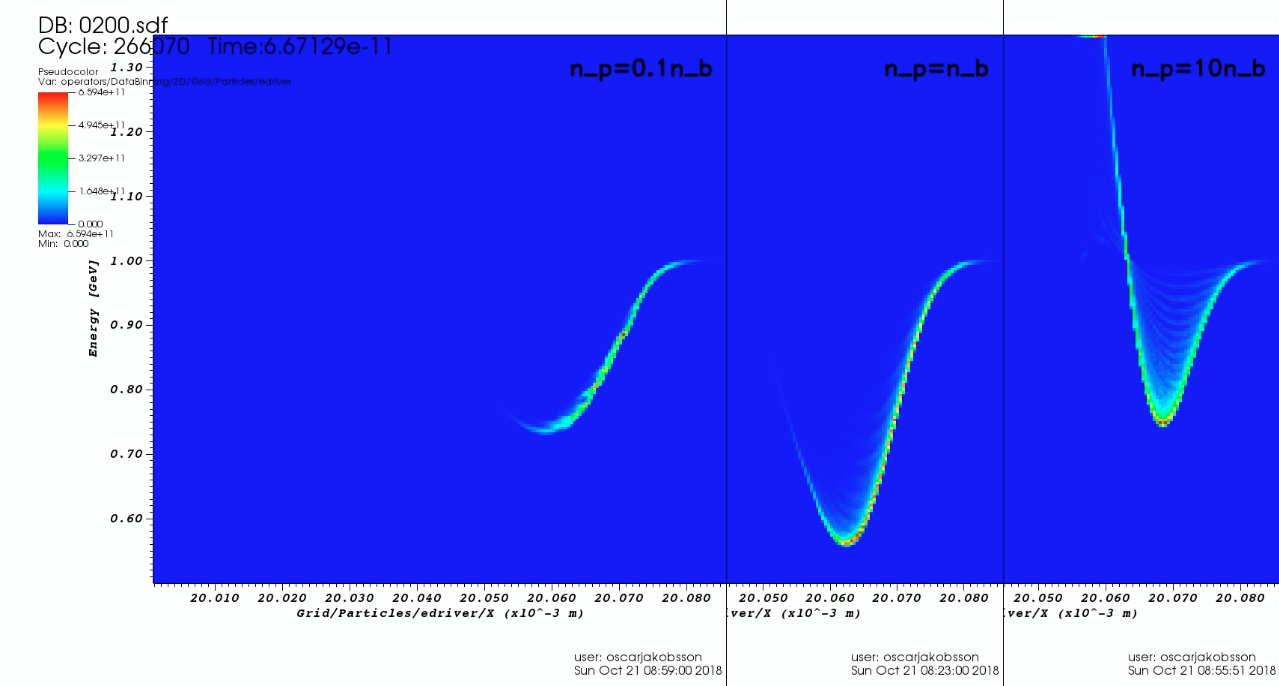
\includegraphics[scale=0.3]{simulation30pc}
\end{figure}
\item[\textcolor{MancPurple}{\textbullet}] By integrating energy histograms using VisIt's query('Integrate') function in a Python script the energy decrease was computed as a function of propagation distance for the 3 cases above:
\begin{figure}[!ht]
\centering
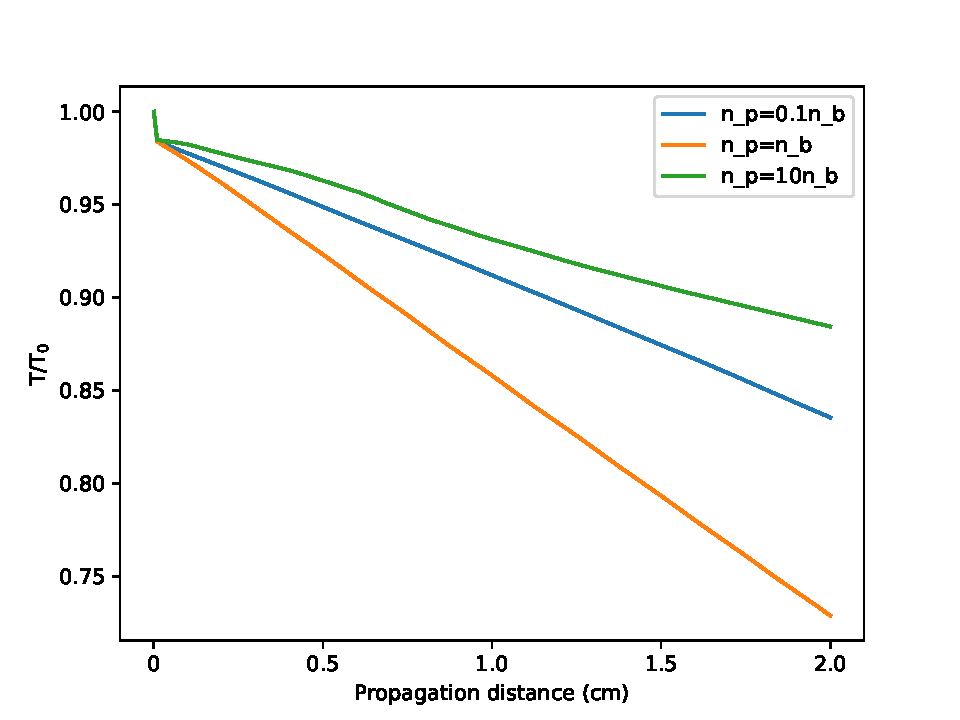
\includegraphics[scale=0.8]{EnergyDecrease30pc.pdf}
\end{figure}
\item[\textcolor{MancPurple}{\textbullet}] The varying plasma density was tried in EPOCH by doing some test simulation. This will be set up and run next week. 
\end{itemize}
\newpage 



\newpage
\section*{Propagation Uniform plasma}
\begin{figure}[!ht]
\centering
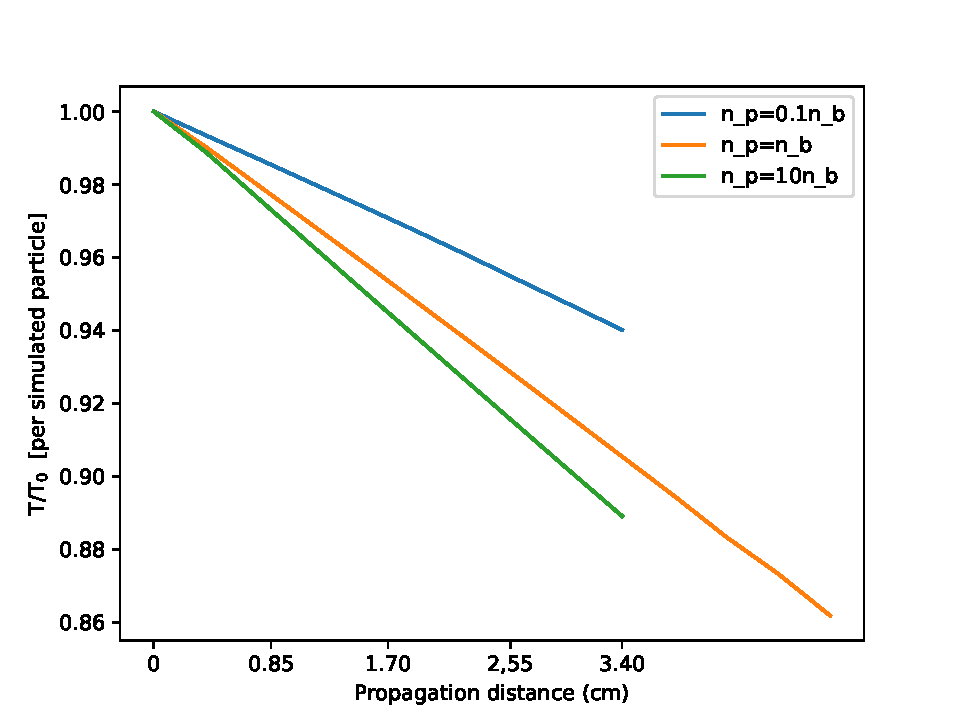
\includegraphics[width=0.75\textwidth]{Energy30pc_per_particle_past_sat_length.pdf}
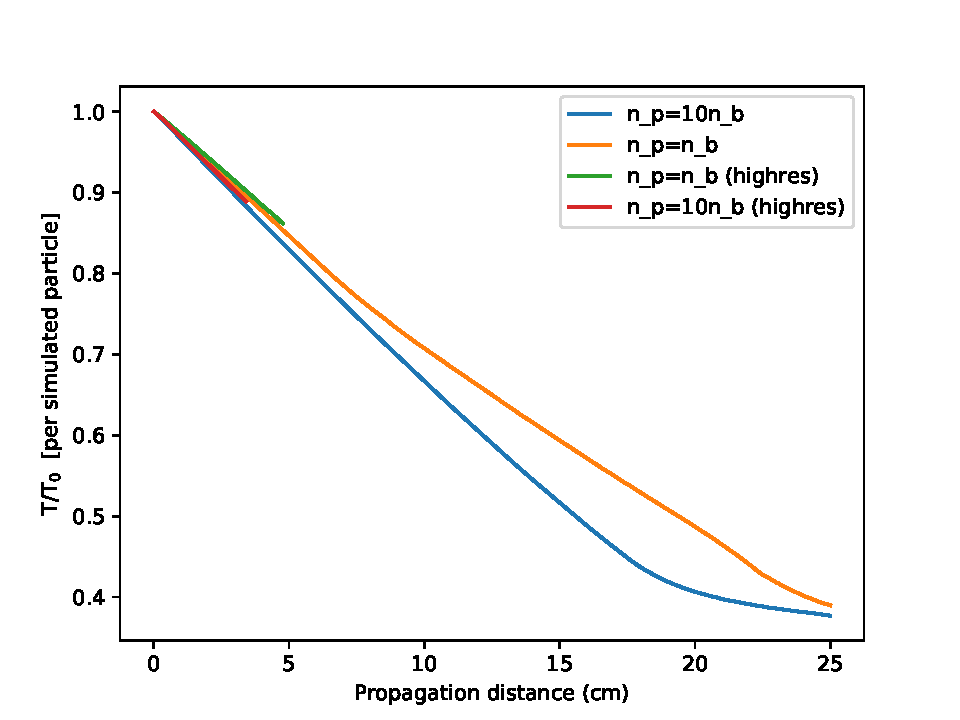
\includegraphics[width=0.75\textwidth]{Energy30pc_per_particle_lowres.pdf}
\end{figure}
\begin{figure}[!ht]
\centering
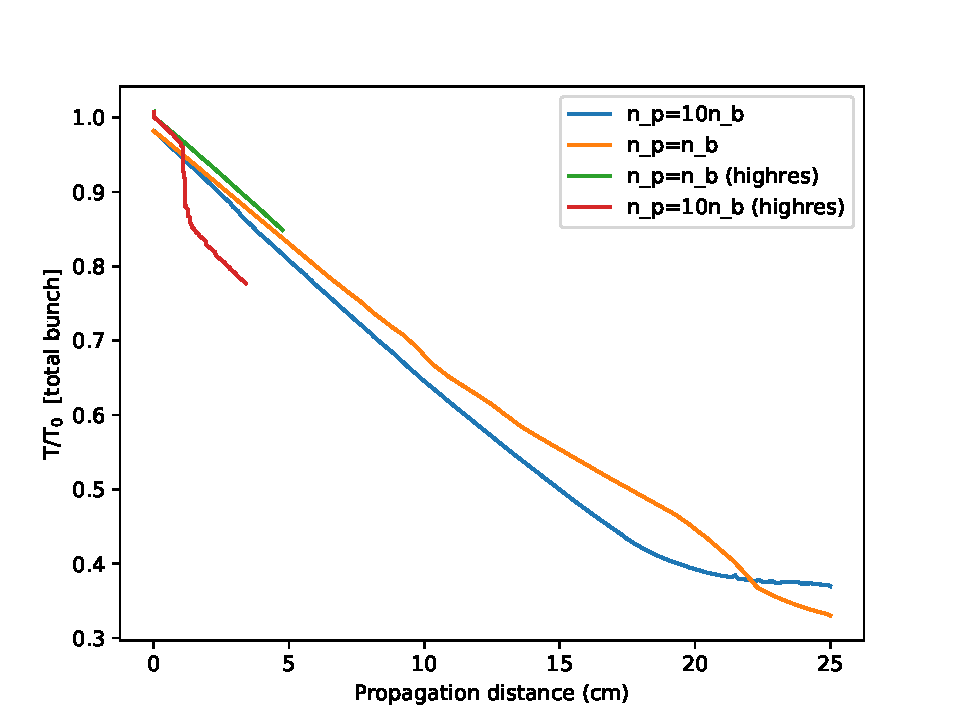
\includegraphics[width=0.78\textwidth]{Energies30pc_lowres.pdf}
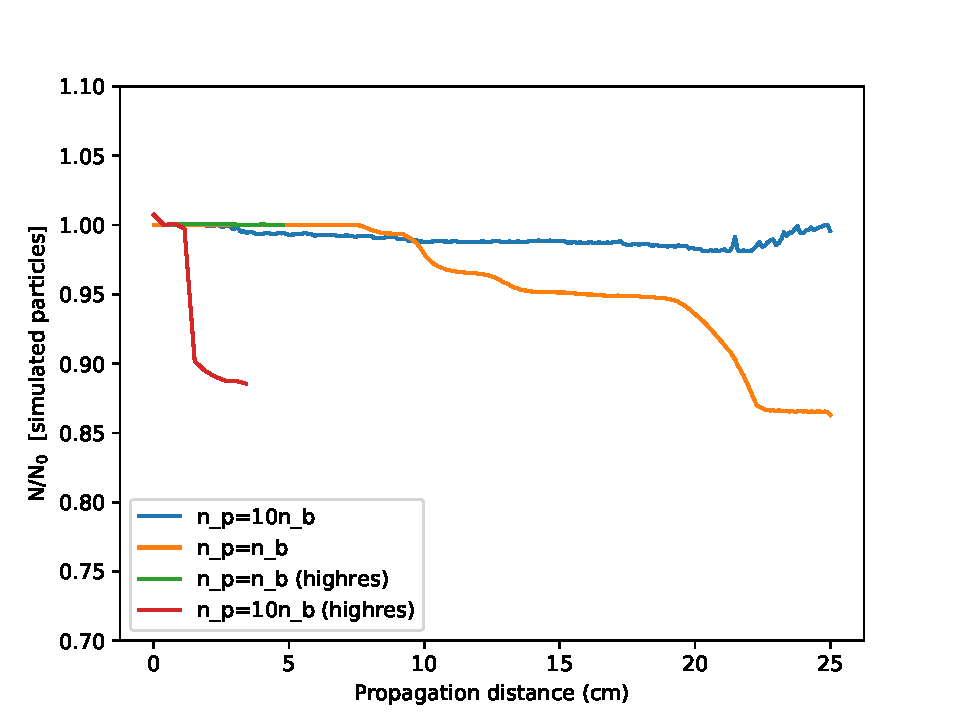
\includegraphics[width=0.78\textwidth]{Particles30pc_lowres.pdf}
\end{figure}


\clearpage
\begin{figure}[!ht]
\centering
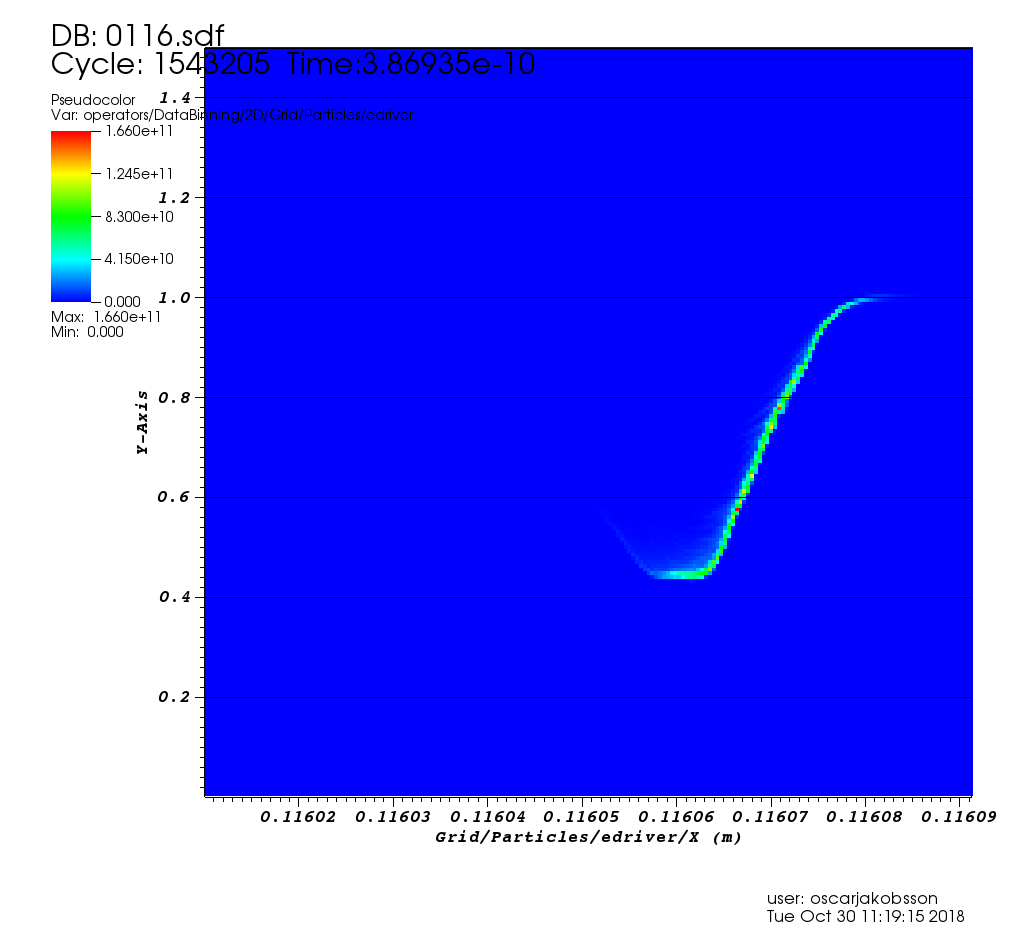
\includegraphics[width=0.49\textwidth]{visit0016.png}
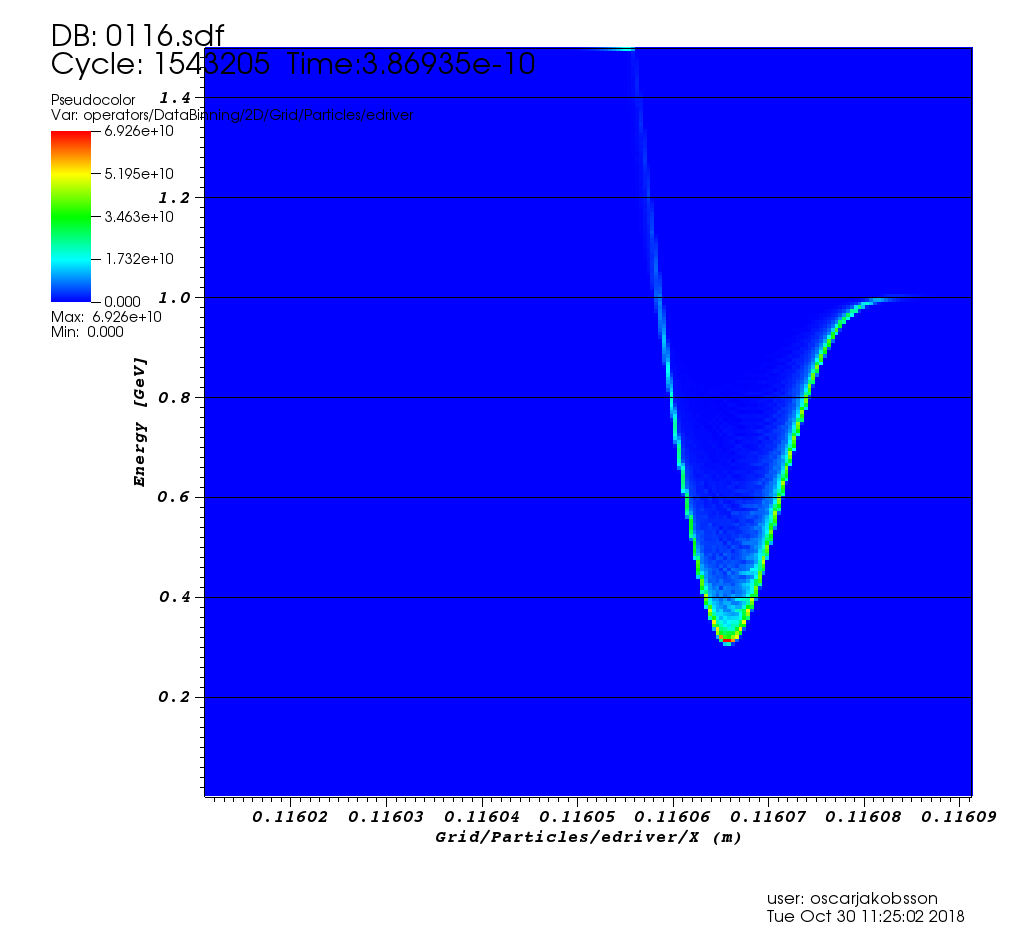
\includegraphics[width=0.49\textwidth]{visit0012.png}
\caption{\textcolor{Orange2}{\textbf{(Left)}}{: Energy distribution for quasilinear case after propagating 11.6 cm} \textcolor{blue}{\textbf{(Right)}}{: Energy distribution for linear case after propagating 11.6 cm.}}
\end{figure}
\begin{figure}[!ht]
\centering
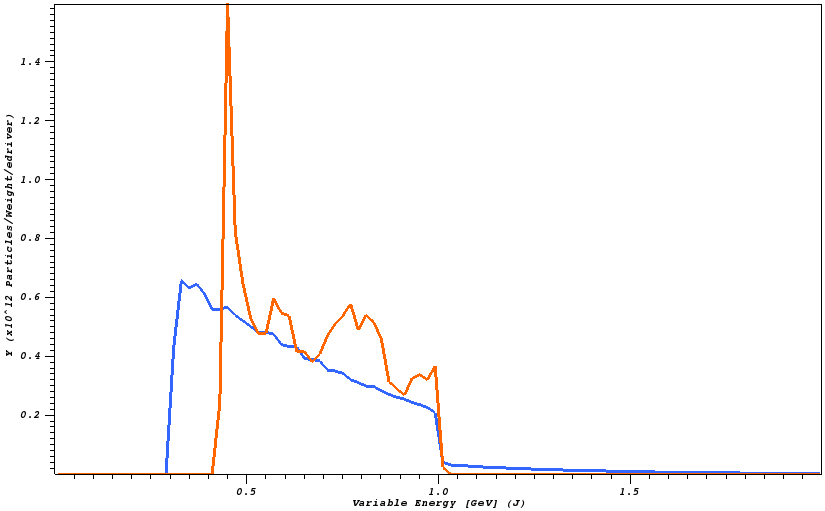
\includegraphics[width=0.9\textwidth]{visit0019.png}
\caption{\textcolor{Orange2}{\textbf{(1)}}{: Quasilinear $n_p=n_b$ after 11.6 cm.} \textcolor{blue}{\textbf{(2)}}{: Linear $n_p=10n_pb$ after 11.6 cm.}}
\end{figure}

\newpage
\begin{figure}[!ht]
\centering
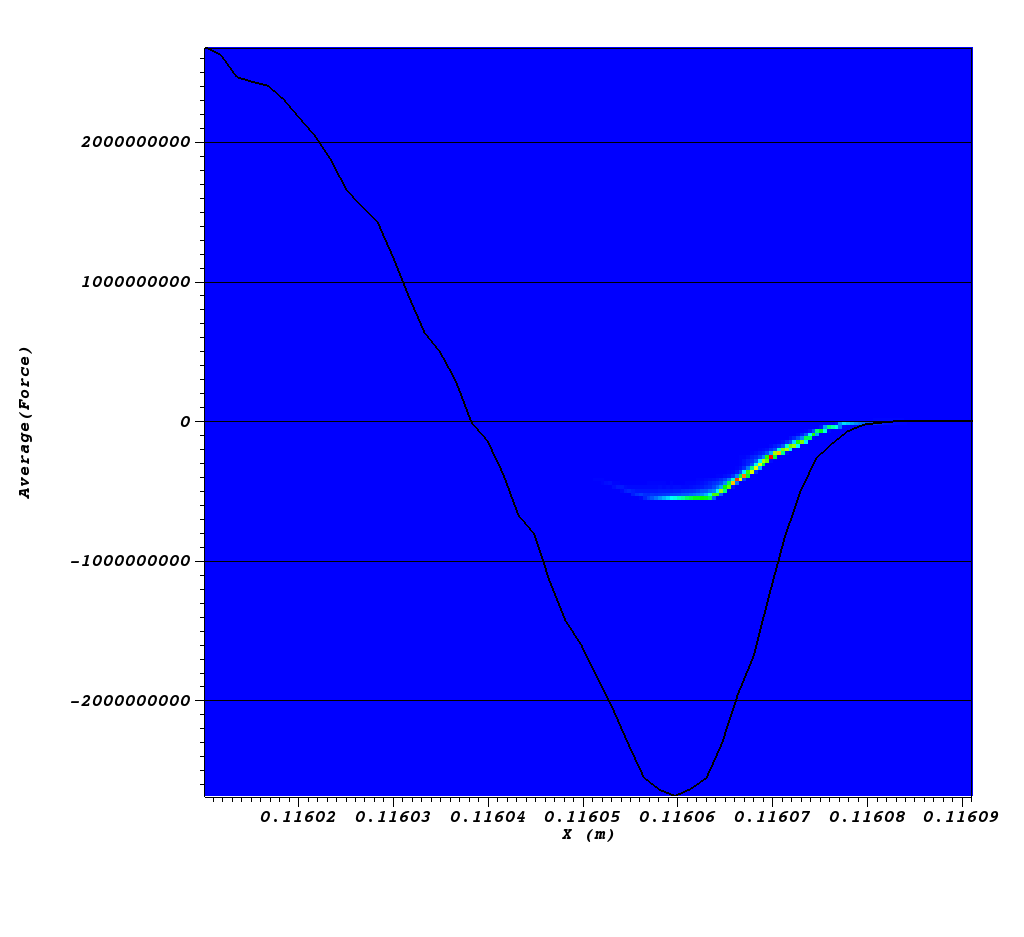
\includegraphics[width=0.6\textwidth]{quasi_energy_force.png}\\
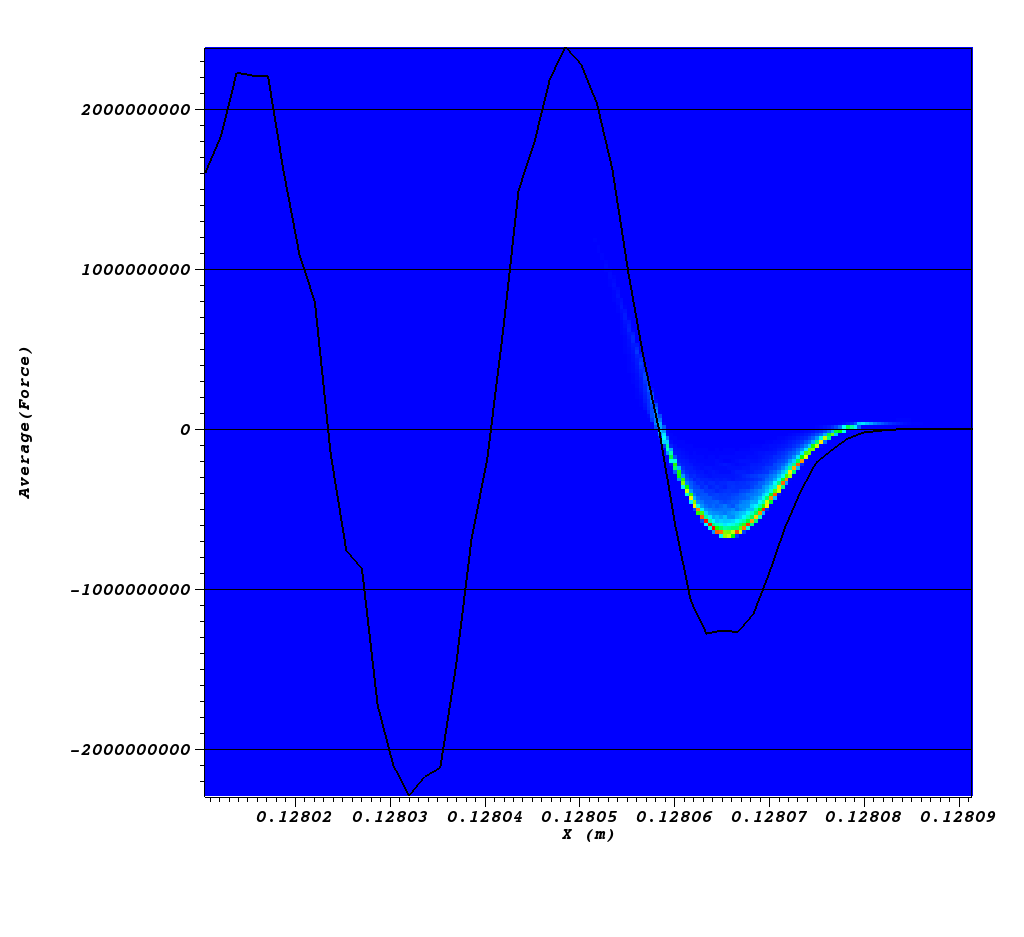
\includegraphics[width=0.6\textwidth]{linear_energy_force.png}
\caption{{\textbf{(Left)}}{: Energy distribution with force for quasilinear case after propagating 11.6 cm} {\textbf{(Right)}}{: Energy distribution with force for linear case after propagating 11.6 cm.}}
\end{figure}

\newpage
\noindent Propagation Uniform plasma.
\begin{figure}[!ht]
\centering
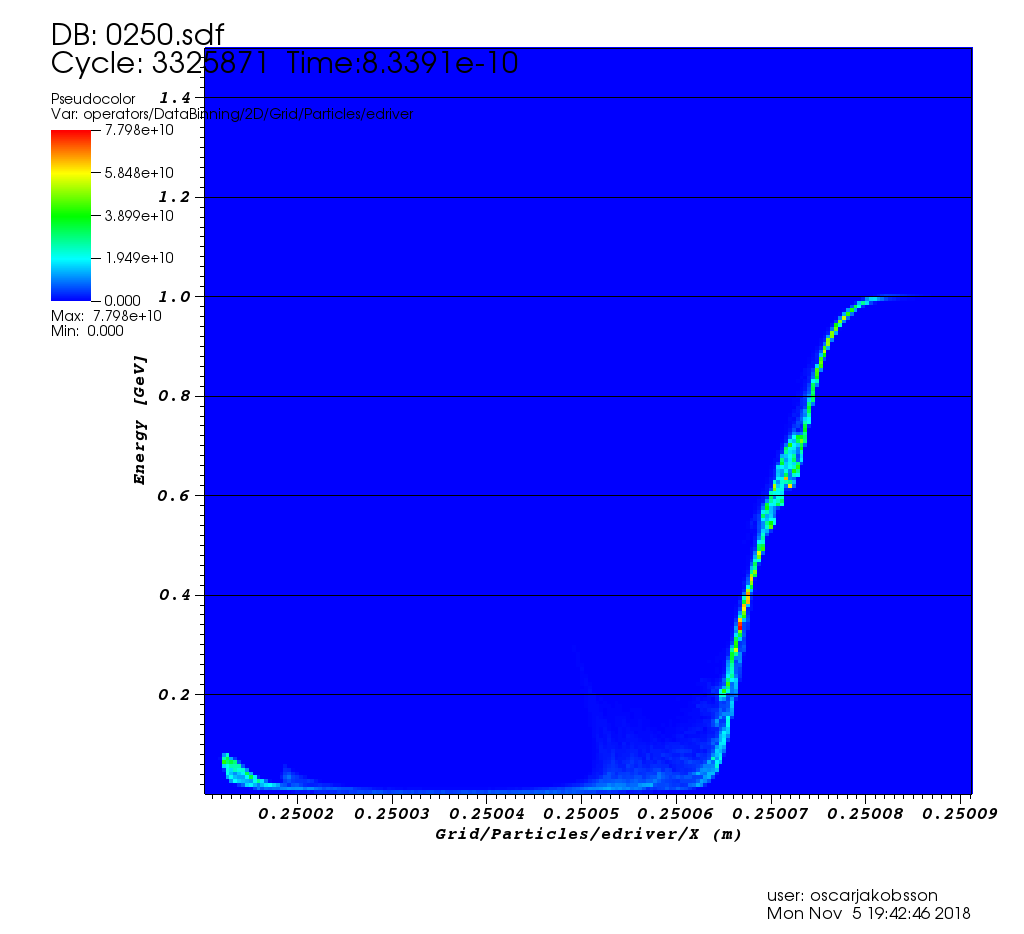
\includegraphics[width=0.49\textwidth]{visit0035.png}
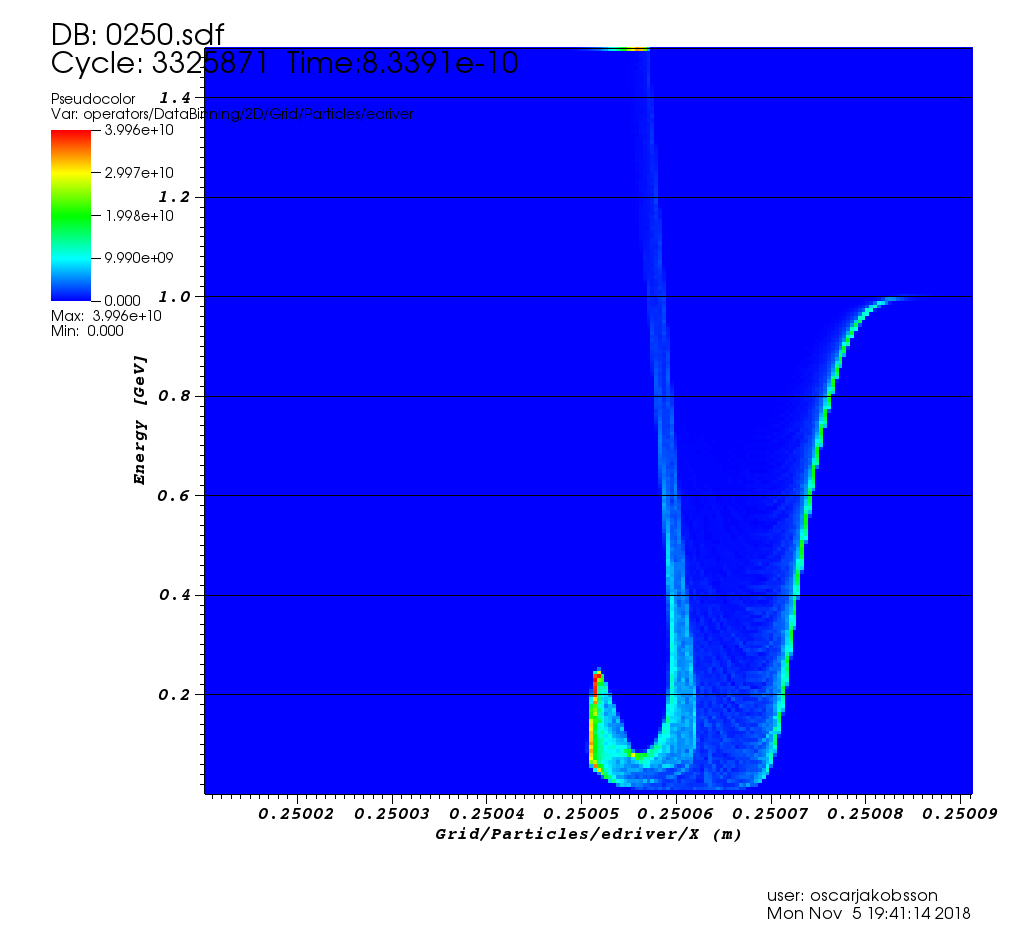
\includegraphics[width=0.49\textwidth]{visit0033.png}
\caption{\textcolor{Orange2}{\textbf{(Left)}}{: Energy distribution for quasilinear case after propagating 25 cm} \textcolor{blue}{\textbf{(Right)}}{: Energy distribution for linear case after propagating 25 cm.}}
\end{figure}
\begin{figure}[!ht]
\centering
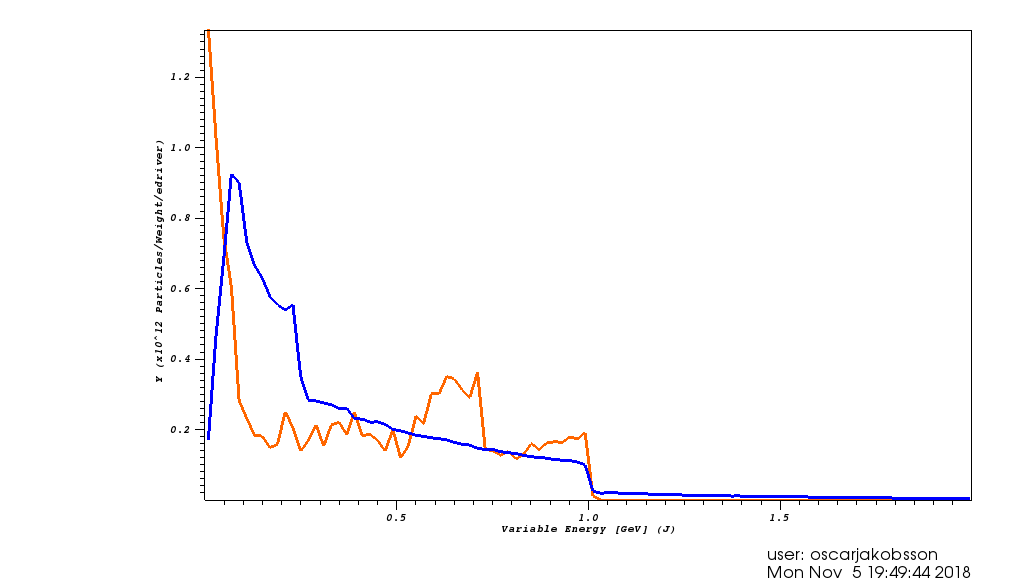
\includegraphics[width=0.9\textwidth]{visit0037.png}
\caption{\textcolor{Orange2}{\textbf{(1)}}{: Quasilinear $n_p=n_b$ after 25 cm.} \textcolor{blue}{\textbf{(2)}}{: Linear $n_p=10n_pb$ after 25 cm.}}
\end{figure}
\begin{figure}[!ht]
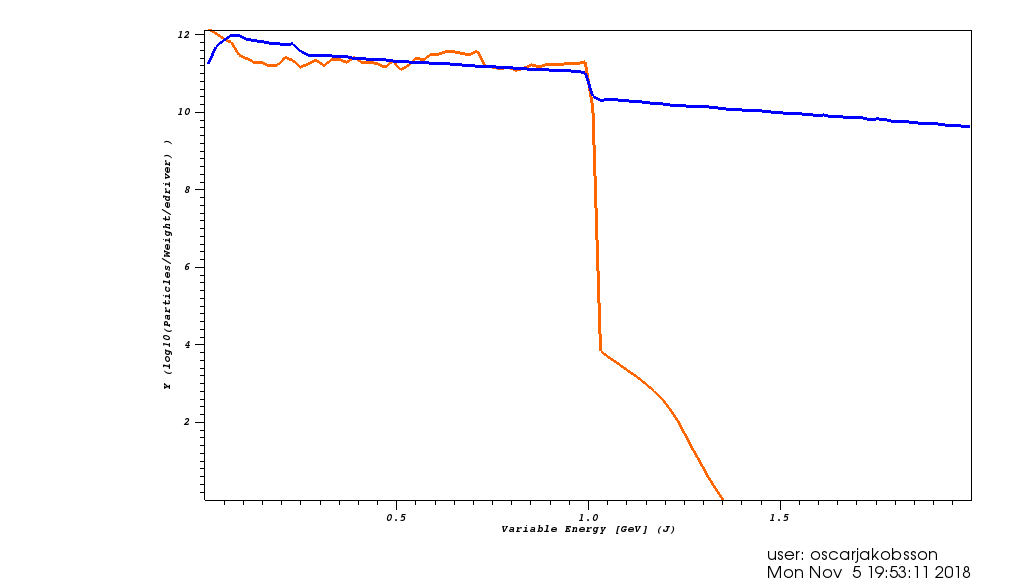
\includegraphics[width=0.9\textwidth]{visit0038.png}
\caption{\textcolor{Orange2}{\textbf{(1)}}{: Quasilinear $n_p=n_b$ after 25 cm.} \textcolor{blue}{\textbf{(2)}}{: Linear $n_p=10n_pb$ after 25 cm.}}
\end{figure}
\begin{figure}[!ht]
\centering
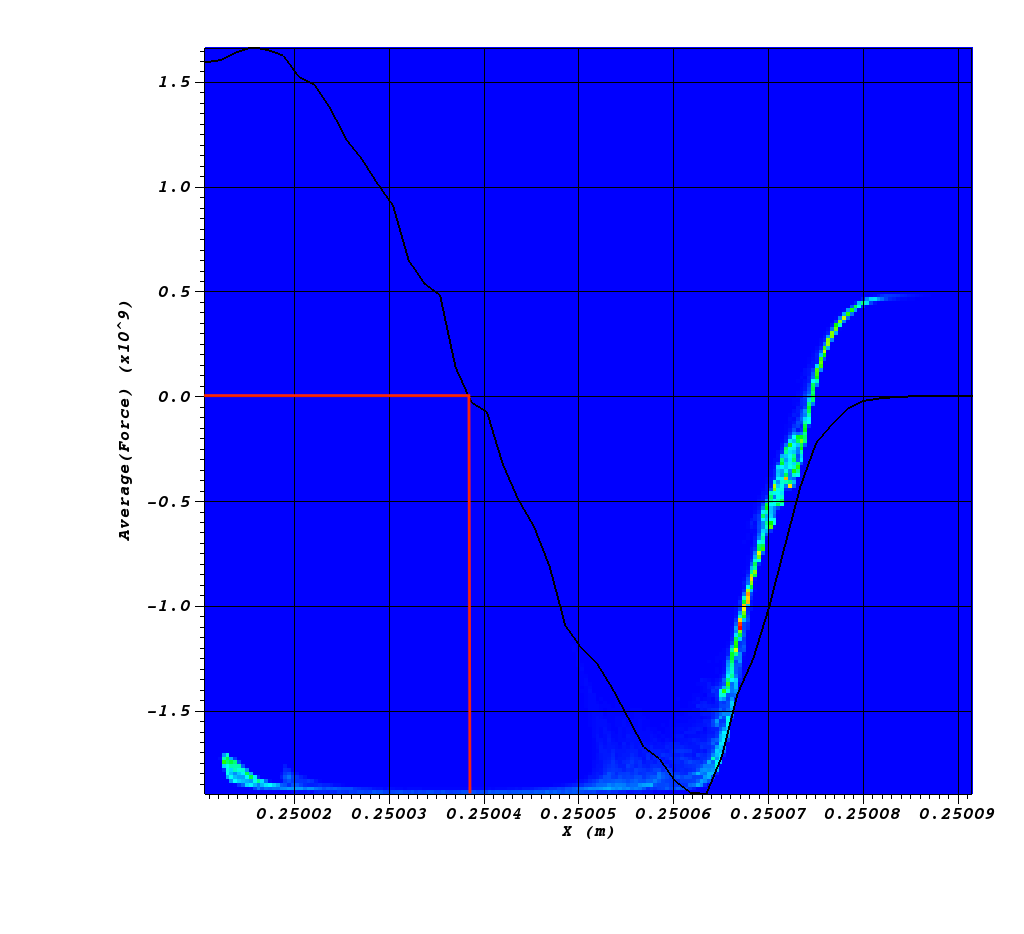
\includegraphics[width=0.49\textwidth]{visit0040.png}
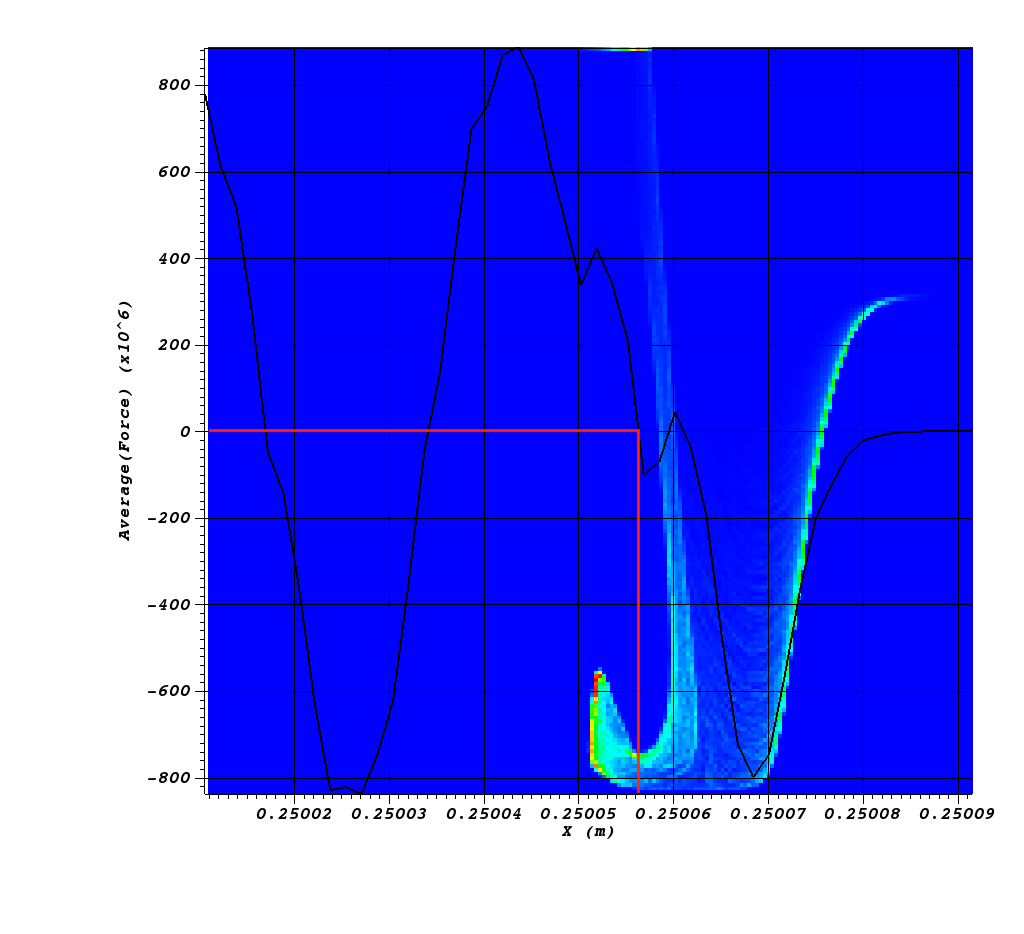
\includegraphics[width=0.49\textwidth]{visit0042.png}
\caption{\textcolor{Orange2}{\textbf{(Left)}}{: Energy distribution with force for quasilinear case after propagating 25 cm} \textcolor{blue}{\textbf{(Right)}}{: Energy distribution with force for linear case after propagating 25 cm}.}
\end{figure}
\clearpage

\begin{figure}[!ht]
\centering
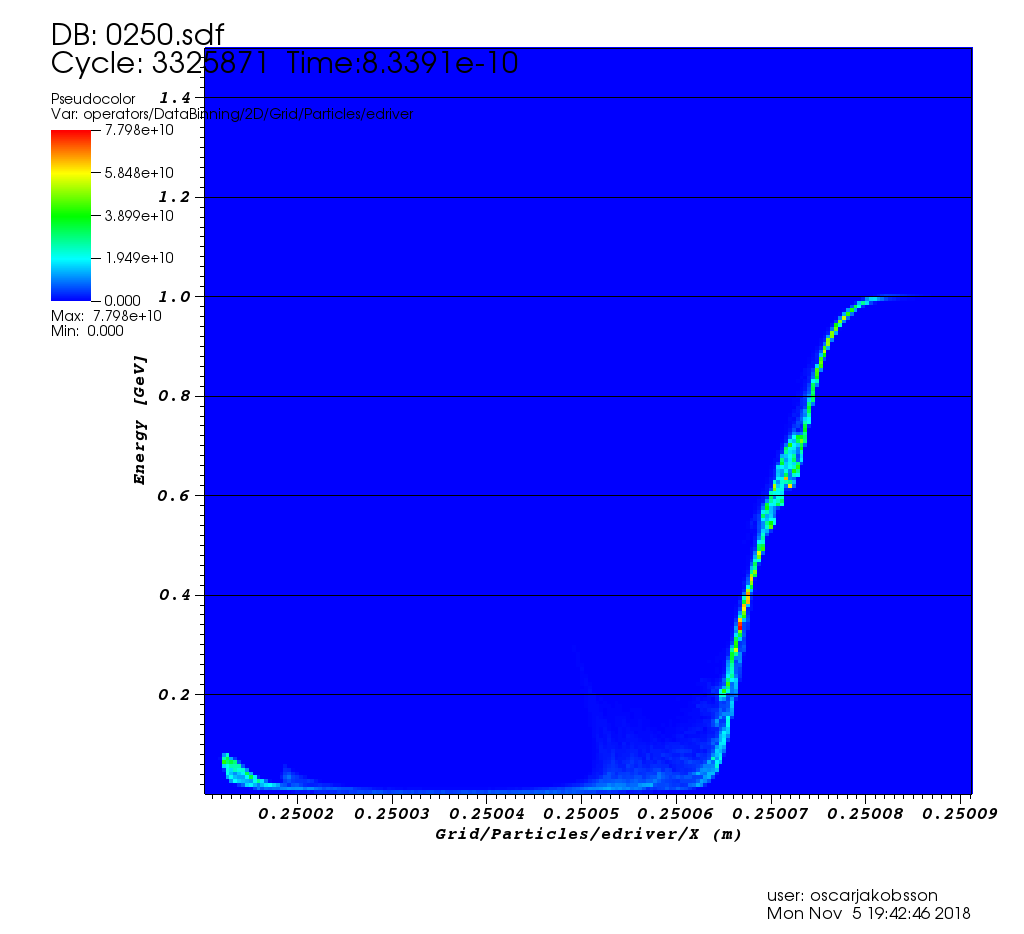
\includegraphics[width=0.49\textwidth]{visit0035.png}
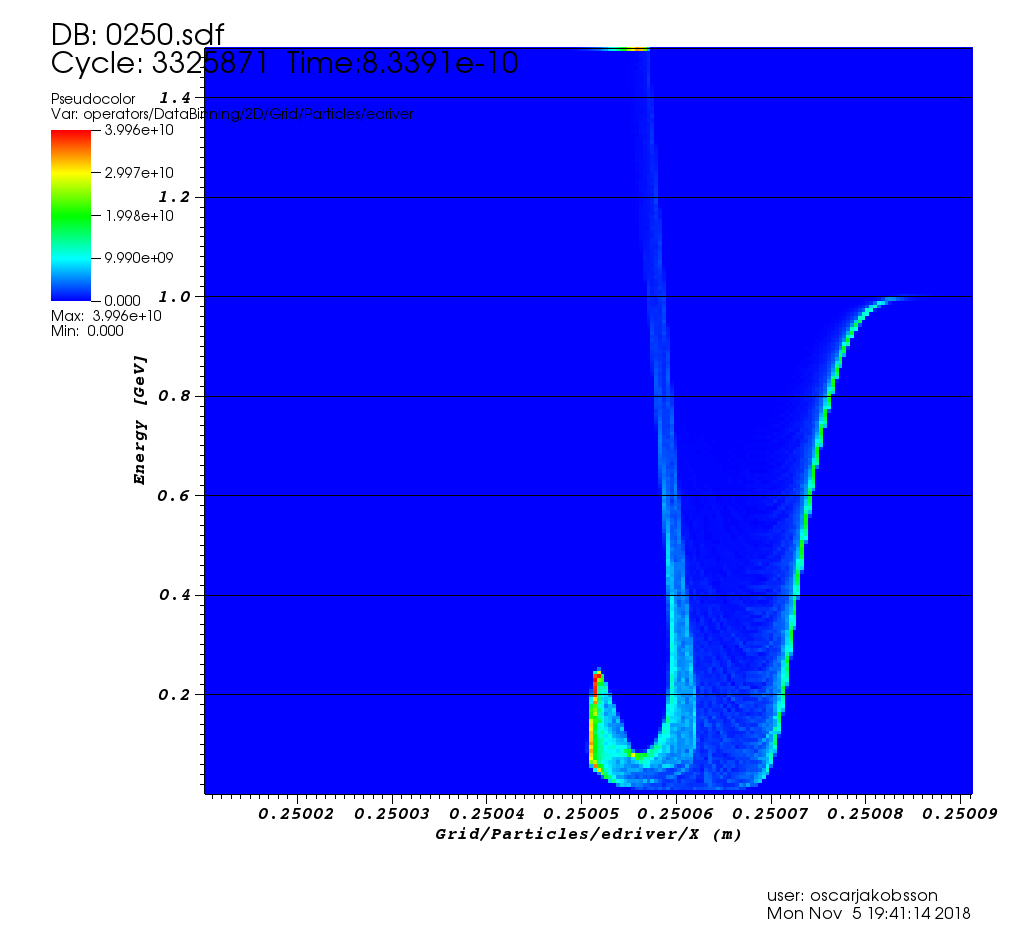
\includegraphics[width=0.49\textwidth]{visit0033.png}
\caption{\textcolor{Orange2}{\textbf{(Left)}}{: Energy distribution for quasilinear case after propagating 25 cm} \textcolor{blue}{\textbf{(Right)}}{: Energy distribution for linear case after propagating 25 cm.}}
\end{figure}
\begin{figure}[!ht]
\centering
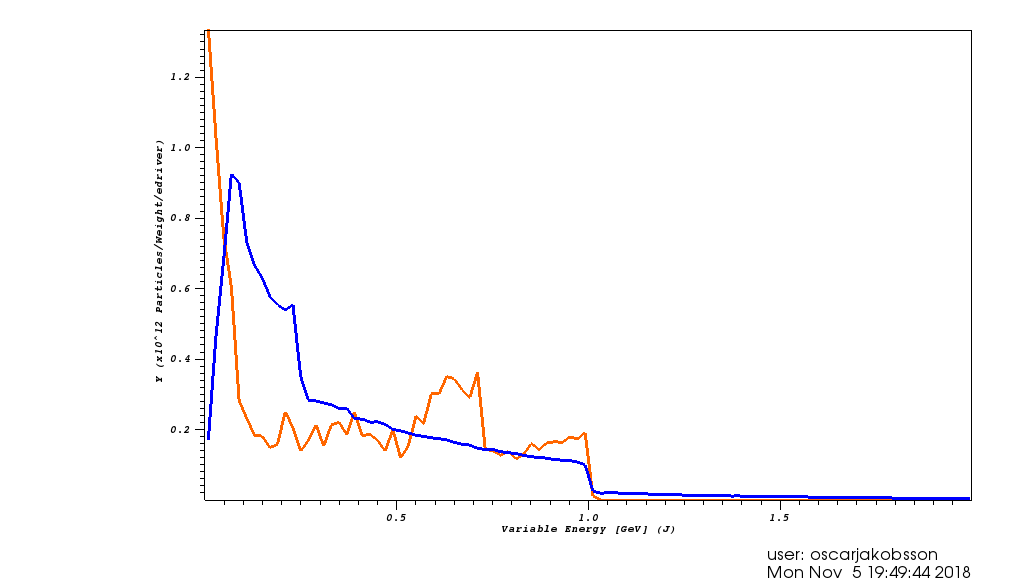
\includegraphics[width=0.9\textwidth]{visit0037.png}
\caption{\textcolor{Orange2}{\textbf{(1)}}{: Histogram energy distribution for quasilinear $n_p=n_b$ after 25 cm.} \textcolor{blue}{\textbf{(2)}}{: Histogram energy distribution for linear $n_p=10n_pb$ after 25 cm.}}
\end{figure}
\clearpage

\begin{figure}[!ht]
\centering
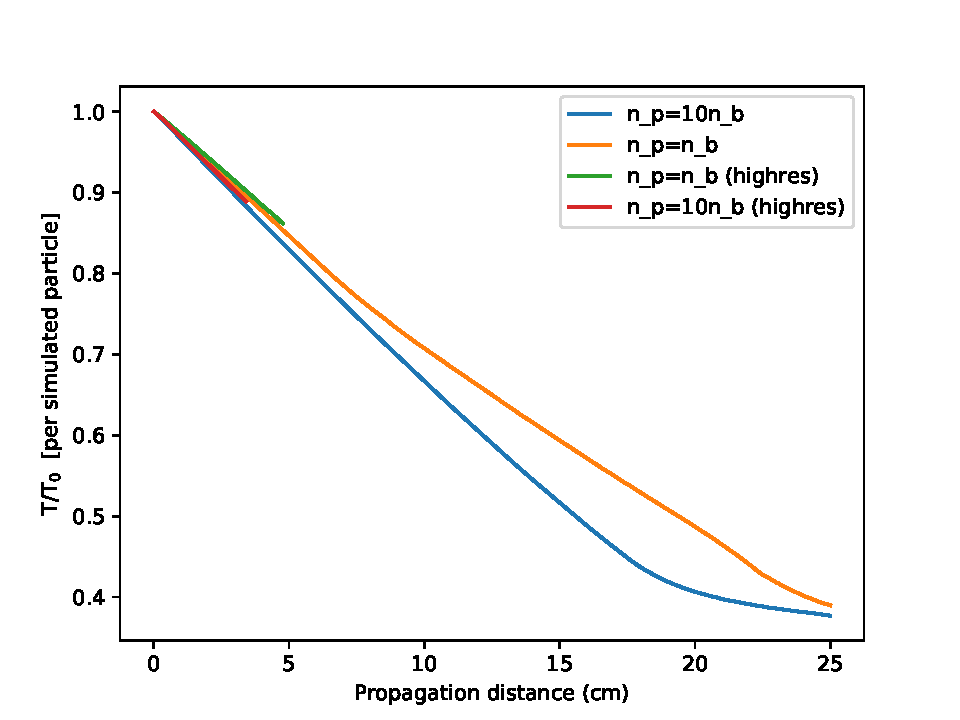
\includegraphics[width=0.75\textwidth]{Energy30pc_per_particle_lowres.pdf}
\end{figure}


\begin{figure}[!ht]
\centering
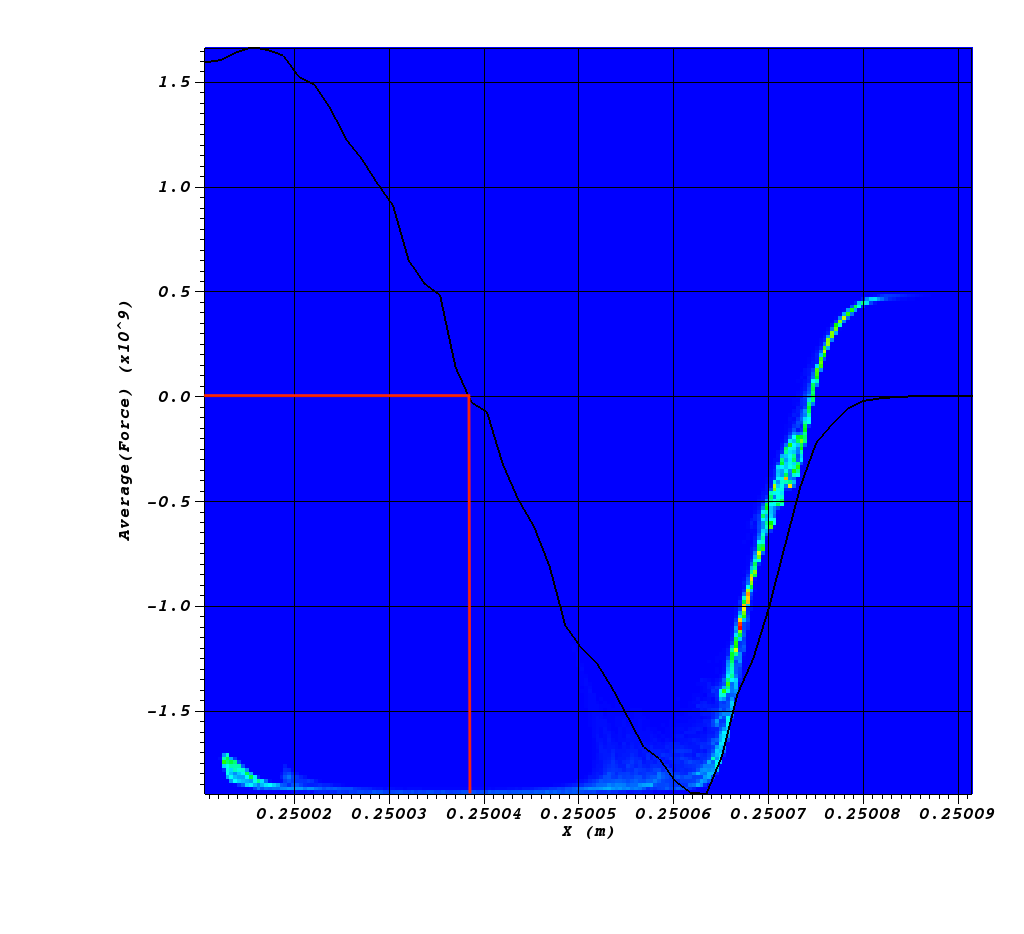
\includegraphics[width=0.49\textwidth]{visit0040.png}
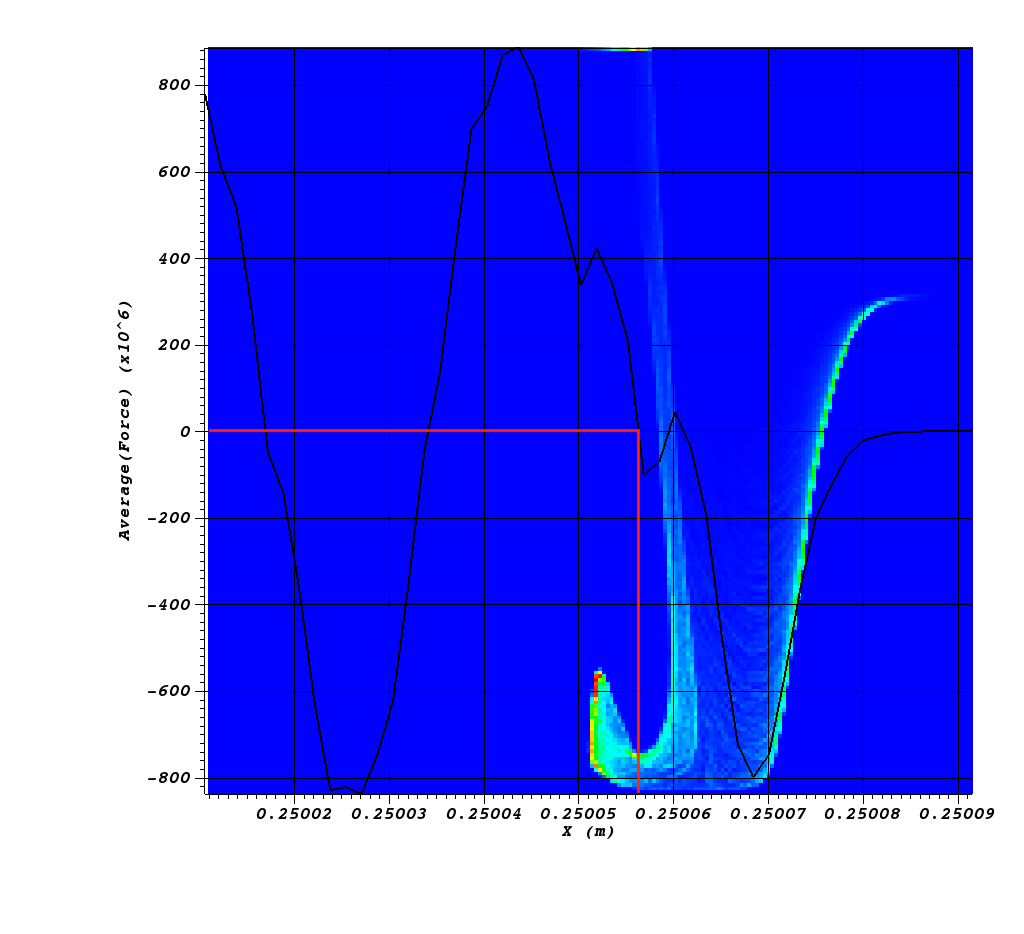
\includegraphics[width=0.49\textwidth]{visit0042.png}
\caption{\textcolor{Orange2}{\textbf{(Left)}}{: Energy distribution with force for quasilinear case after propagating 25 cm} \textcolor{blue}{\textbf{(Right)}}{: Energy distribution with force for linear case after propagating 25 cm}.}
\end{figure}
\clearpage
\begin{figure}[!ht]
\centering
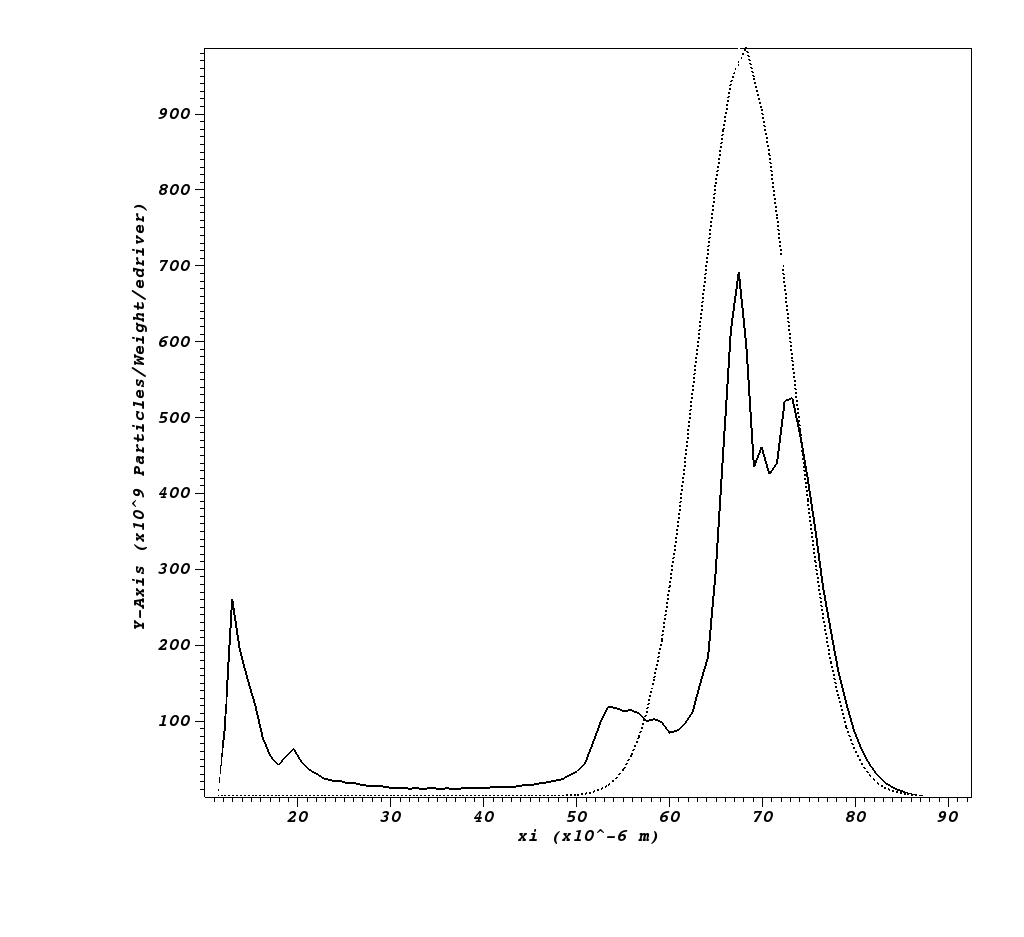
\includegraphics[width=0.66\textwidth]{25cm_lengthdist_start_end.png}\vspace{-20pt}\\
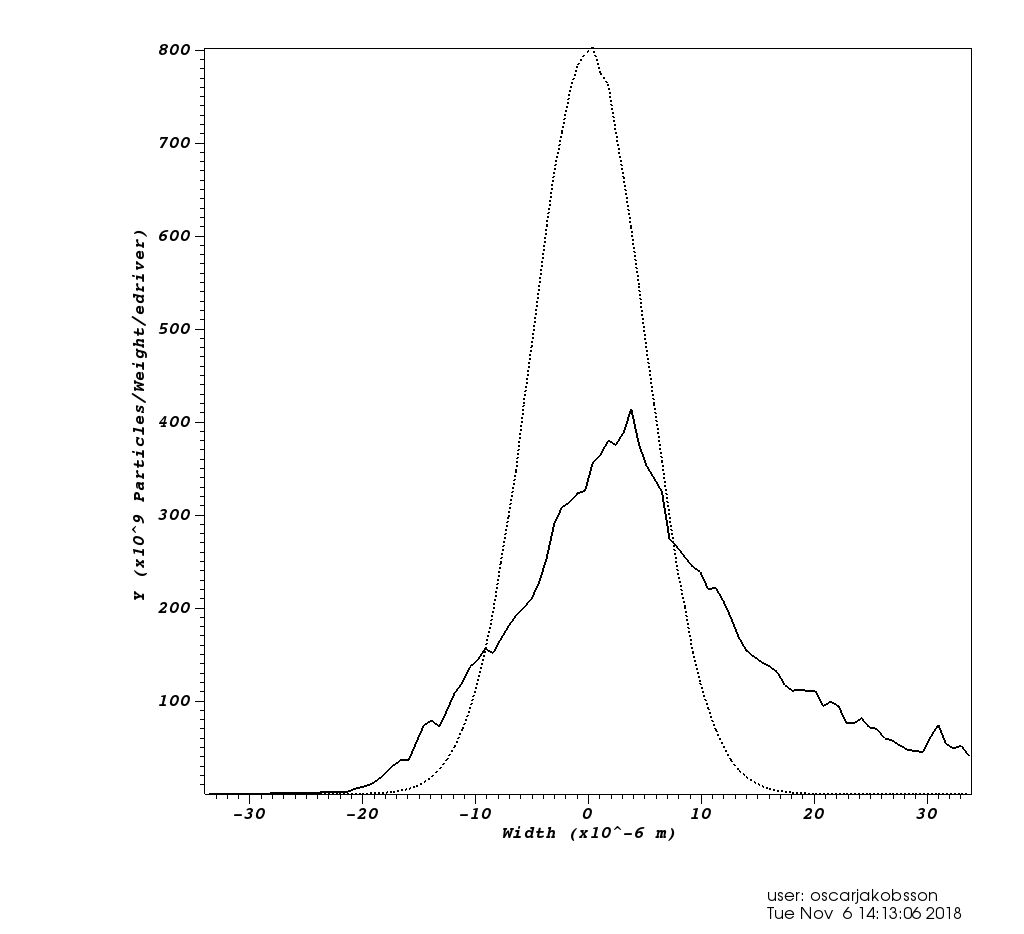
\includegraphics[width=0.66\textwidth]{25cm_widthdist_start_end.png}
\caption{{\textbf{(Left)}}{: Bunch length distribution for quasilinear case after propagating 0 cm (dotted) and 25 cm (solid)}. {\textbf{(Right)}}{: Bunch width distribution for quasilinear case after propagating 0 cm (dotted) and 25 cm (solid)}.}
\end{figure}

\clearpage


\noindent \textbf{Success!} Managed to set up an initial distribution with arbitrary energy distribution. 
\begin{figure}[!ht]
\centering
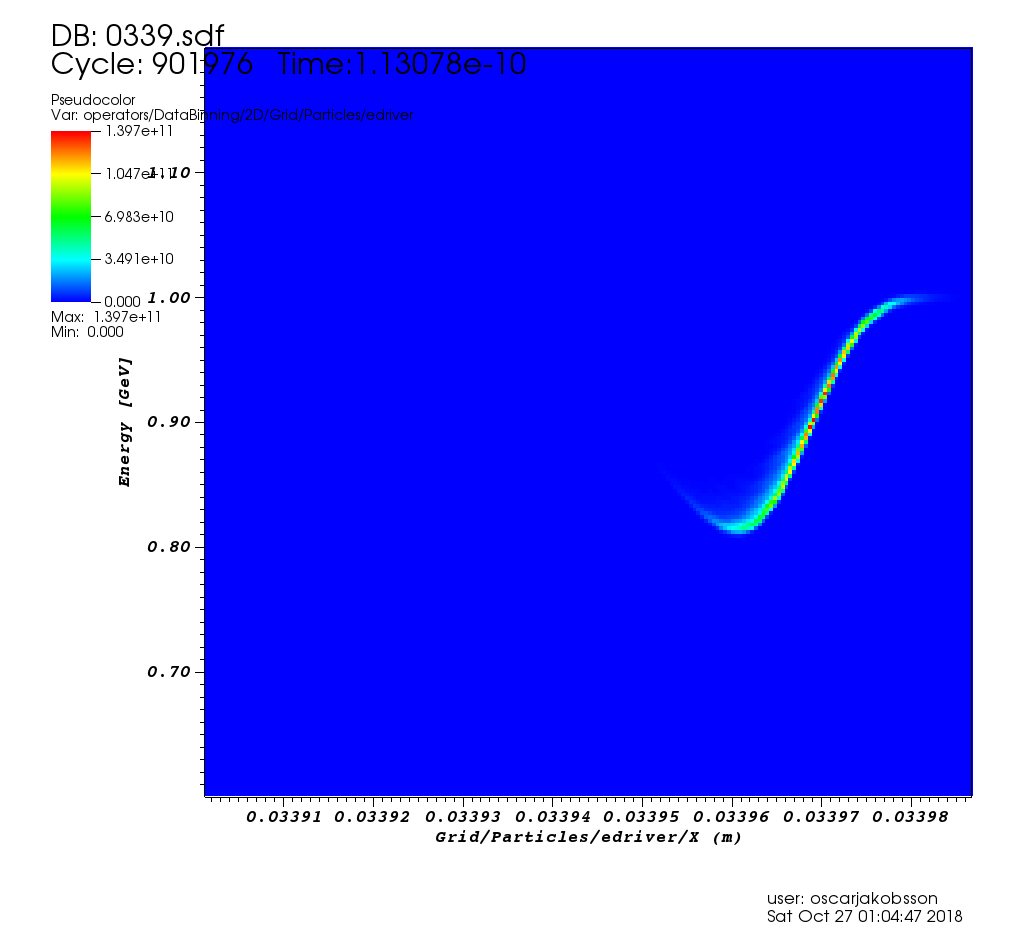
\includegraphics[width=0.49\textwidth]{visit0002.png}
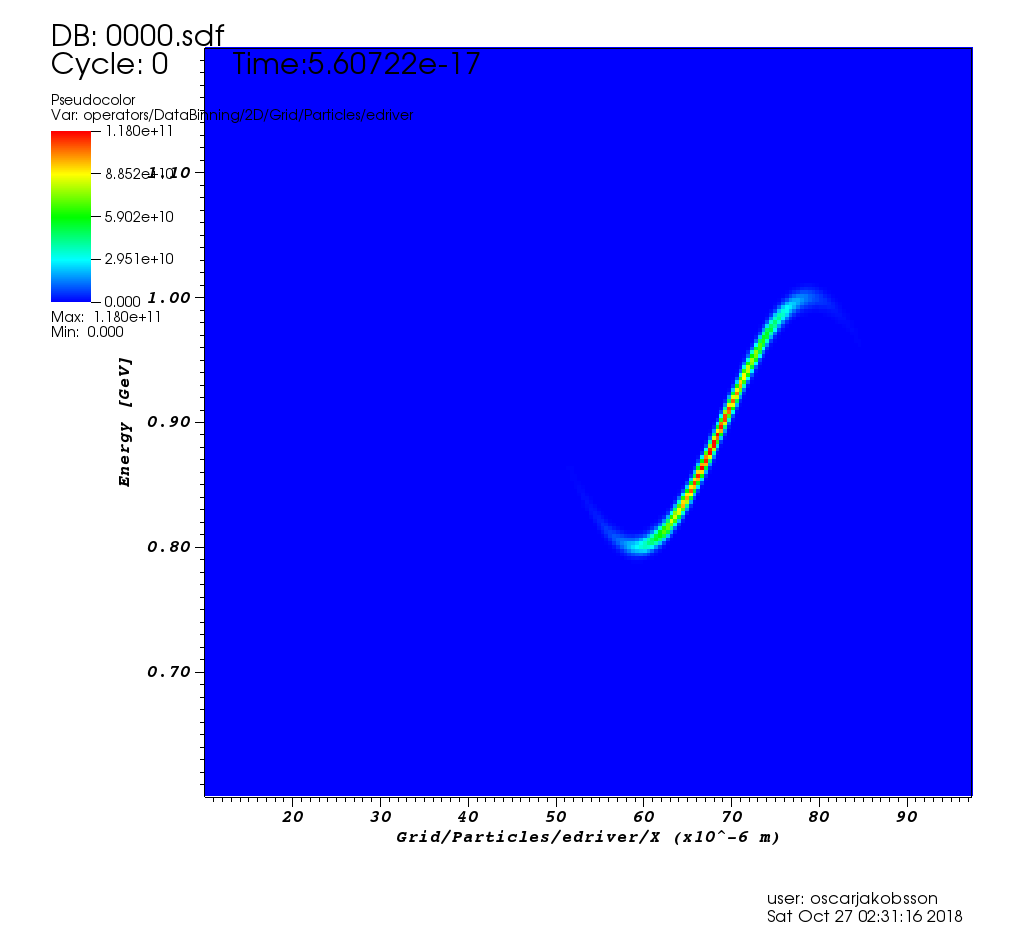
\includegraphics[width=0.49\textwidth]{visit0007.png}
\caption{\textcolor{Orange2}{\textbf{(Left)}}{: Energy distribution for bunch after propagating 3.4cm} \textcolor{blue}{\textbf{(Right)}}{: Energy distribution for bunch initialised at start of simulation.}}
\end{figure}
\begin{figure}[!ht]
\centering
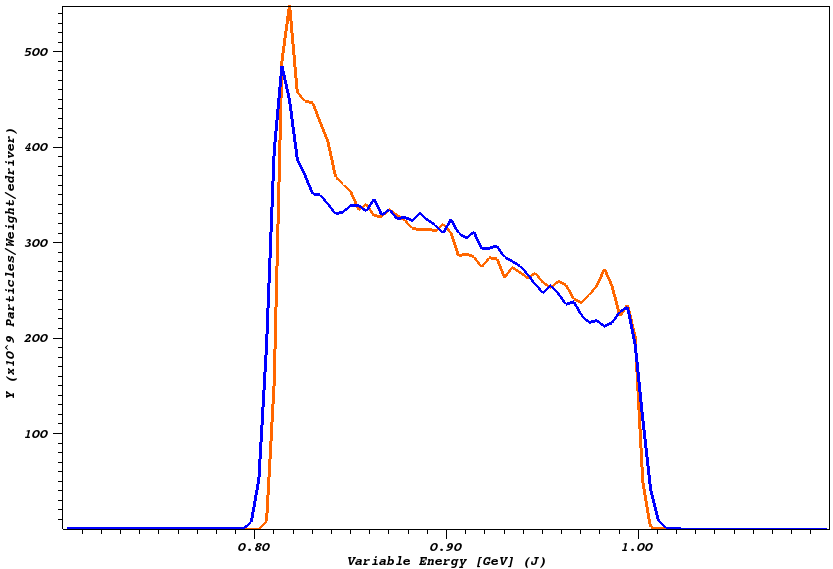
\includegraphics[width=0.8\textwidth]{visit0004.png}
\caption{\textcolor{Orange2}{\textbf{(1)}}{: Energy distribution for bunch after propagating 3.4cm} \textcolor{blue}{\textbf{(2)}}{: Energy distribution for bunch initialised at start of simulation.}}
\end{figure}

\clearpage

\begin{figure}[!ht]
\centering
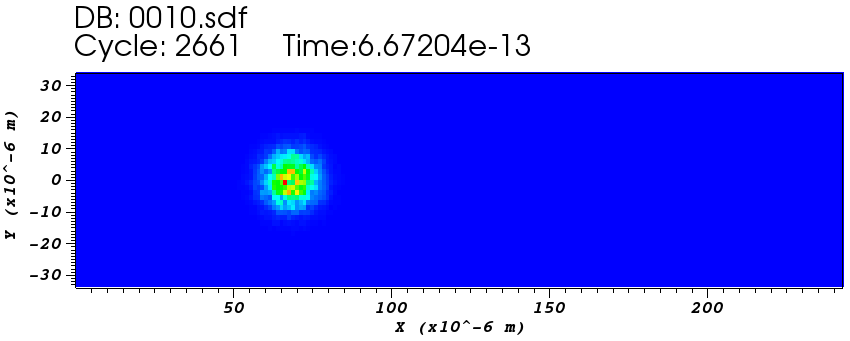
\includegraphics[width=0.7\textwidth]{buncht1copy.png}\\
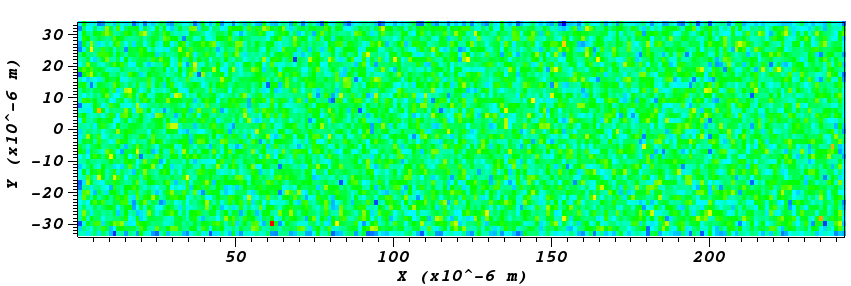
\includegraphics[width=0.7\textwidth]{lasert1copy.png}
\caption{Time: $t_1$. (Upper) edriver density, (Lower) electron plasma density}
\vspace{-10pt}
\end{figure}
\begin{figure}[!ht]
\centering
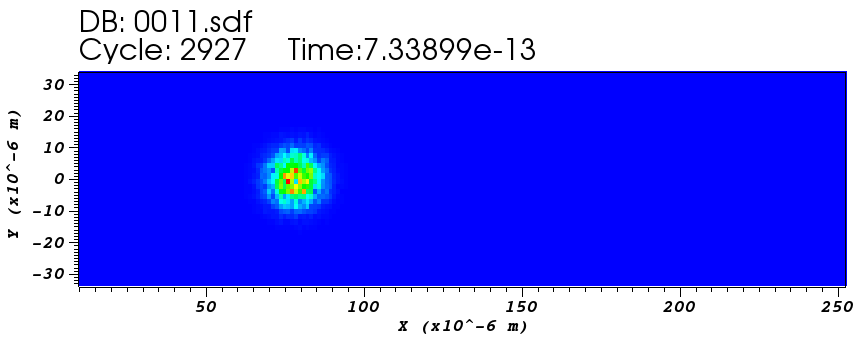
\includegraphics[width=0.7\textwidth]{buncht2copy.png}\\
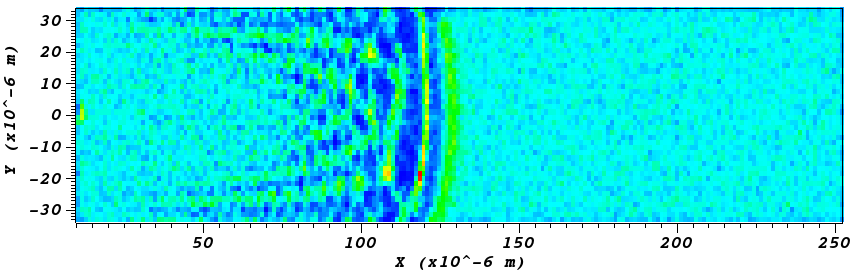
\includegraphics[width=0.7\textwidth]{lasert2copy.png}
\caption{Time: $t_2$. (Upper) edriver density, (Lower) electron plasma density when laser has appeared at $\sim 120 \mu$m}
\end{figure}












\clearpage
 \vfill
 \bibliographystyle{unsrt}
 \bibliography{PWFA.bib}


 \end{document}
 